\documentclass[11pt]{article}

\usepackage[margin=1in]{geometry}
\usepackage{booktabs}
\usepackage{graphicx}
\usepackage{hyperref}
\usepackage{listings}
\usepackage{microtype}
\usepackage{parskip}
\usepackage[section]{placeins}
\usepackage{tikz}
\usepackage{url}
\usepackage{xcolor}
\usetikzlibrary{arrows.meta,positioning}

\hypersetup{
    colorlinks=true,
    linkcolor=blue!50!black,
    citecolor=blue!50!black,
    urlcolor=blue!50!black
}

\lstset{
    basicstyle=\ttfamily\small,
    breaklines=true,
    frame=single,
    backgroundcolor=\color{gray!5},
    columns=fullflexible
}

\title{\textbf{Learning State Transitions in Infrastructure Logs for Anomaly Detection}}
\author{
Satheesh Kumar G R\\
San Jose State University\\
\texttt{satheeshkumar.geetharavi@sjsu.edu}
}
\date{}

\begin{document}
\maketitle

\begin{abstract}
Modern software systems generate logs and traces for almost every action they perform. These records are useful for debugging, but they are hard to monitor with only hand-written rules. Many failures are not just ``CPU is high'' or ``status is error.'' Sometimes the issue is that the system moves through an unusual sequence of states. This project studies a simple idea: learn normal state transitions from infrastructure logs, then treat surprising next states as possible anomalies. A practical gap in existing log-anomaly work is that results are often reported for one dataset or one preprocessing setup, so it is hard to know whether the model is learning useful system behavior or just benefiting from the way the data was prepared. To address that gap, I compare RNN, LSTM, and Transformer models across OpenStack, OpenStack2k, HDFS2k, and GAIA MicroSS traces. The focus is on how model choice, dataset type, state representation, and evaluation setup change the final anomaly-detection behavior.
\end{abstract}

\section{Introduction}

Infrastructure systems produce a lot of logs. A single application can generate logs from API servers, databases, caches, background workers, and load balancers. In a cloud system, there are also traces that show which service called which other service. These logs are usually full of key-value style information: service name, status code, event id, component name, latency, instance id, request id, and message text.

Engineers usually monitor these systems using dashboards, queries, and alert rules. This works when the problem is obvious. For example, if error rate is greater than 10\%, send an alert. But many real problems are not that simple. A log line can look normal by itself, but become suspicious because of where it appears in the sequence.

The main idea in this project is to learn how normal system states usually transition. Instead of writing a separate rule for every possible failure, the model sees previous log states and predicts what should happen next. If the next state is surprising, that transition gets a high anomaly score. In simple terms, the project asks whether sequence models can learn normal state transitions in infrastructure logs and detect anomalies as deviations from expected behavior.

This is similar in spirit to DeepLog \cite{du2017deeplog}, but I use it as a framework for comparing datasets, model architectures, and feature choices. The final system compares RNN, LSTM, and Transformer models and also tests a product-infrastructure trace dataset, GAIA MicroSS. This matters because the practical question is not only whether a model can work on one dataset, but whether the same idea still makes sense when the log format, labels, and available fields change.

\section{Example of Anomaly and Use Cases}

The easiest way to understand the problem is with examples. In many systems, one row alone is not enough. The problem is the relationship between fields or the order of events.

\begin{lstlisting}[caption={Example transition anomalies in key-value style logs}]
--- Cross-field behavior anomaly ---

service=payment status=200 latency=30 retry=0
service=payment status=200 latency=35 retry=0
service=payment status=200 latency=32 retry=8

The status still says success, but retry=8 is strange.


--- Service path anomaly ---

service=cache hit=true latency=5
service=cache hit=true latency=6
service=database query=true latency=40

After repeated cache hits, a database query suddenly appears.


--- Trace anomaly ---

service=web endpoint=/login status=200 duration=80ms
service=web endpoint=/login status=200 duration=90ms
service=web endpoint=/login status=500 duration=2000ms

The endpoint is the same, but the behavior changes.
\end{lstlisting}

In these examples, a manually written rule may miss the issue unless the engineer already knows what combination to check. A learning model can instead learn common transitions and assign high surprise to unusual ones.

\section{Related Work and Gap}

Traditional anomaly detection methods use thresholds, statistical tests, clustering, or distribution-based checks \cite{chandola2009survey}. These methods are useful, but they usually need manually selected features. They also do not naturally understand sequence order.

Earlier log-mining work showed that logs contain repeated structure and useful system behavior patterns \cite{xu2009consolelogs,lou2010invariants}. Deep learning methods later started modeling logs as sequences. DeepLog predicts the next log key and flags unexpected events \cite{du2017deeplog}. LogAnomaly adds semantic and quantitative information \cite{meng2019loganomaly}. LogBERT uses Transformer-style masked prediction for log anomaly detection \cite{guo2021logbert}. Surveys also point out that log anomaly detection is very sensitive to preprocessing, labels, and dataset choice \cite{landauer2023dlsurvey}.

The gap I focus on is practical: even if the model idea is simple, the result can change a lot depending on how logs are represented, how labels are defined, and which fields are included. This project is not claiming to invent a brand-new neural architecture. The contribution is a clear comparison of state-transition learning across multiple infrastructure datasets, with extra attention to feature choices and evaluation pitfalls.

\section{Proposed Approach}

\subsection{State Representation}

Each log or trace row is converted into a compact state token. A state token is just a string that represents the important fields for that row. Later, the string is mapped to an integer id so the neural network can use it.

The conversion has three steps:

\begin{quote}
raw row $\rightarrow$ keep stable useful fields $\rightarrow$ normalize changing values $\rightarrow$ state token
\end{quote}

Here are examples of what that looks like for each dataset:

\begin{lstlisting}[caption={Examples of converting raw dataset rows into state tokens}]
--- OpenStack ---
Raw row:
component=nova.compute.claims
level=INFO
content="[instance: 3f8a...] disk limit not specified"

State token:
nova.compute.claims | INFO | [instance: <uuid>] disk limit not specified


--- OpenStack2k ---
Raw row:
component=nova.osapi_compute.wsgi.server
level=INFO
event_id=E25

State token:
nova.osapi_compute.wsgi.server | INFO | E25


--- HDFS2k ---
Raw row:
event_id=E10
content="PacketResponder 1 for block blk_1073741825 terminating"

State token:
E10 | PacketResponder <*> for block blk_<*> terminating


--- GAIA MicroSS ---
Raw row:
service=webservice1
endpoint=/web_login_service
status=200
duration=394ms
message="request call function webservice1.web_login_service"

State token:
webservice1 | /web_login_service | duration=<500ms |
request call function webservice1.web_login_service
\end{lstlisting}

I normalize unstable values like UUIDs, block ids, and IP addresses because otherwise every request id or block id becomes a new unique state. That would make the vocabulary too large and would not help the model learn general behavior.

\subsection{Next-State Prediction}

After creating state tokens, I build sliding windows. If the sequence length is 5, the model sees 5 previous states and predicts the next state.

\[
x_t = [s_{t-5}, s_{t-4}, s_{t-3}, s_{t-2}, s_{t-1}], \qquad y_t = s_t
\]

If the model expects state A but the actual state is rare or unexpected, the loss becomes high. This high loss is used as the anomaly score.

\subsection{How the Models Work}

\textbf{RNN.} The RNN is the simplest model. It reads the sequence one state at a time and keeps a hidden memory. It is a good baseline because it can learn short transition patterns without much complexity.

\textbf{LSTM.} The LSTM is like an improved RNN. It has gates that decide what to remember and what to forget. This should help when the important context happened several steps earlier.

\textbf{Transformer.} The Transformer uses attention. Instead of only passing information step by step, it can compare all states in the window with each other. This can help when the anomaly depends on relationships between non-adjacent states.

\subsection{Anomaly Score}

The model is trained with cross-entropy loss. In simple terms, loss means how surprised the model is by the true next state.

\[
A(x_t, y_t) = -\log p_\theta(y_t \mid x_t)
\]

Low loss means the transition looked normal. High loss means the transition was surprising. After training, I choose a threshold on validation data. If the anomaly score is above the threshold, the window is predicted as anomalous.

\section{Methodology Diagram}

Figure \ref{fig:method} shows the full workflow. This is the same overall idea from the proposal, but updated for the final experiments.

\begin{figure}[!htbp]
\centering
\resizebox{0.98\textwidth}{!}{%
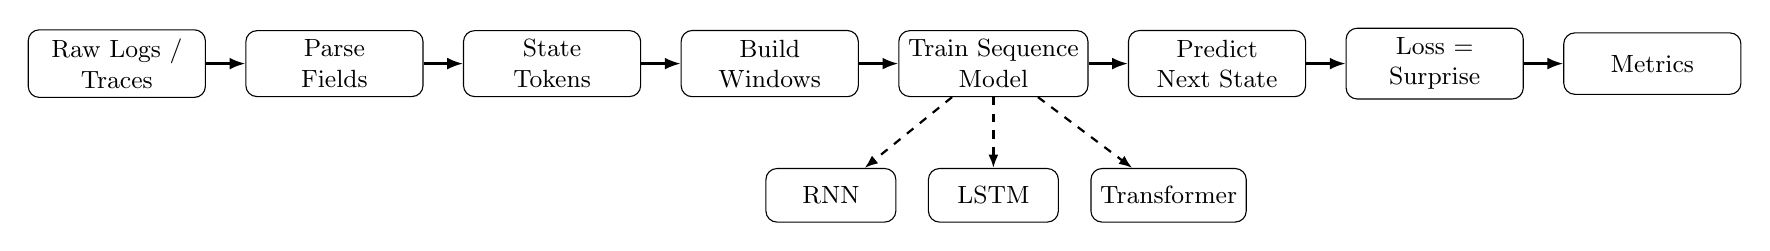
\begin{tikzpicture}[
    node distance=7mm and 5mm,
    box/.style={draw, rounded corners, align=center, minimum width=2.25cm, minimum height=0.78cm, font=\small},
    modelbox/.style={draw, rounded corners, align=center, minimum width=1.65cm, minimum height=0.68cm, font=\small},
    arrow/.style={-{Latex[length=2.0mm]}, thick},
    choice/.style={-{Latex[length=1.7mm]}, thick, dashed}
]
\node[box] (data) {Raw Logs /\\Traces};
\node[box, right=of data] (prep) {Parse\\Fields};
\node[box, right=of prep] (state) {State\\Tokens};
\node[box, right=of state] (seq) {Build\\Windows};
\node[box, right=of seq] (model) {Train Sequence\\Model};
\node[box, right=of model] (pred) {Predict\\Next State};
\node[box, right=of pred] (score) {Loss =\\Surprise};
\node[box, right=of score] (eval) {Metrics};

\node[modelbox, below=9mm of model] (lstm) {LSTM};
\node[modelbox, left=4mm of lstm] (rnn) {RNN};
\node[modelbox, right=4mm of lstm] (trf) {Transformer};

\draw[arrow] (data) -- (prep);
\draw[arrow] (prep) -- (state);
\draw[arrow] (state) -- (seq);
\draw[arrow] (seq) -- (model);
\draw[arrow] (model) -- (pred);
\draw[arrow] (pred) -- (score);
\draw[arrow] (score) -- (eval);
\draw[choice] (model) -- (rnn);
\draw[choice] (model) -- (lstm);
\draw[choice] (model) -- (trf);
\end{tikzpicture}%
}
\caption{Architecture and evaluation workflow for state-transition anomaly detection.}
\label{fig:method}
\end{figure}

\section{Datasets}

I used four dataset settings. Table \ref{tab:datasets} gives the high-level summary, and Table \ref{tab:samples} shows what one example state looks like from each dataset.

\begin{table}[!htbp]
\centering
\caption{Datasets used in the project.}
\label{tab:datasets}
\begin{tabular}{@{}llll@{}}
\toprule
Dataset & Source & Sequence unit & Label type \\
\midrule
OpenStack & Loghub full archive & VM instance & Real sparse labels \\
OpenStack2k & Loghub structured sample & Log stream & Controlled anomalies \\
HDFS2k & Loghub structured sample & Log stream & Block-derived labels \\
GAIA & MicroSS traces & Web-service trace stream & Non-200 status labels \\
\bottomrule
\end{tabular}
\end{table}

\begin{table}[!htbp]
\centering
\caption{Representative examples from each dataset.}
\label{tab:samples}
\small
\begin{tabular}{@{}p{0.15\textwidth}p{0.27\textwidth}p{0.48\textwidth}@{}}
\toprule
Dataset & Fields used & Example state \\
\midrule
OpenStack &
component, level, normalized content &
\texttt{nova.compute.claims | INFO | [instance: <uuid>] disk limit not specified} \\
\addlinespace
OpenStack2k &
component, level, event id &
\texttt{nova.osapi\_compute.wsgi.server | INFO | E25} \\
\addlinespace
HDFS2k &
event id from template &
\texttt{E10 | PacketResponder <*> for block blk\_<*> terminating} \\
\addlinespace
GAIA MicroSS &
service, endpoint, duration, message &
\texttt{webservice1 | /web\_login\_service | duration=<500ms | request call function} \\
\bottomrule
\end{tabular}
\end{table}

OpenStack is closest to the original infrastructure-log problem, but its anomaly labels are very sparse. OpenStack2k is useful as a sanity check because controlled anomalies can be injected. HDFS2k is a small standard log-anomaly sample. GAIA is useful because it feels closer to product infrastructure: services, endpoints, durations, messages, and status codes.

\section{Metrics Explained}

The metrics can be confusing, so I explain them here.

\textbf{Accuracy} means how often the model predicted the exact next state correctly. This is useful, but it is not enough for anomaly detection.

\textbf{Precision} asks: out of everything the model flagged as anomaly, how many were actually anomaly? High precision means fewer false alarms.

\textbf{Recall} asks: out of all real anomalies, how many did the model catch? High recall means fewer missed problems.

\textbf{F1 score} balances precision and recall. It is useful when anomalies are rare, which is common in logs.

\textbf{AUC} measures whether anomalous examples usually receive higher anomaly scores than normal examples. AUC around 0.5 is close to random. AUC close to 1.0 means strong separation.

For this project, F1 and AUC are more important than next-event accuracy, because the goal is anomaly detection, not just predicting common events.

\section{Experiments}

The experiments were designed to answer a few simple questions:

\begin{itemize}
    \item Does the basic state-transition idea work?
    \item Do RNN, LSTM, and Transformer behave differently?
    \item Does sequence length matter?
    \item Does larger model capacity help?
    \item What happens if a feature directly reveals the label?
\end{itemize}

The main grid uses:

\begin{itemize}
    \item sequence length: 5, 10, 15;
    \item embedding dimension: 32 or 64;
    \item hidden dimension: 64 or 128;
    \item model depth: 1 or 2 layers;
    \item models: RNN, LSTM, Transformer.
\end{itemize}

For OpenStack, OpenStack2k, and HDFS2k, the focused grid has 45 runs. For GAIA, I ran 15 more runs on a 20,000-row subset of webservice traces. I also ran a GAIA ablation where status code was first included and then removed from the input state.

The code for loading datasets, building state tokens, training the models, running the experiment grid, and regenerating the report figures is available at:

\begin{center}
\url{https://github.com/satheesh18/log_anomaly_detection}
\end{center}

\section{Results}

\subsection{Best Model Results}

Table \ref{tab:results} shows the best result for each dataset/model pair.

\begin{table}[!htbp]
\centering
\caption{Best result for each dataset/model pair.}
\label{tab:results}
\small
\begin{tabular}{@{}llrrrrr@{}}
\toprule
Dataset & Model & Acc. & Prec. & Recall & F1 & AUC \\
\midrule
HDFS2k & RNN & 0.387 & 0.250 & 0.286 & 0.267 & 0.544 \\
HDFS2k & LSTM & 0.361 & 0.273 & 0.214 & 0.240 & 0.555 \\
HDFS2k & Transformer & 0.328 & 0.150 & 0.214 & 0.176 & 0.560 \\
\midrule
OpenStack & RNN & 0.986 & 0.022 & 0.567 & 0.043 & 0.526 \\
OpenStack & LSTM & 0.986 & 0.022 & 0.500 & 0.042 & 0.558 \\
OpenStack & Transformer & 0.986 & 0.021 & 0.433 & 0.040 & 0.527 \\
\midrule
OpenStack2k & RNN & 0.406 & 0.468 & 0.710 & 0.564 & 0.915 \\
OpenStack2k & LSTM & 0.397 & 0.579 & 0.355 & 0.440 & 0.922 \\
OpenStack2k & Transformer & 0.497 & 0.400 & 0.710 & 0.512 & 0.930 \\
\midrule
GAIA no-status & RNN & 0.391 & 0.130 & 0.319 & 0.184 & 0.567 \\
GAIA no-status & LSTM & 0.394 & 0.106 & 0.405 & 0.167 & 0.554 \\
GAIA no-status & Transformer & 0.412 & 0.128 & 0.339 & 0.186 & 0.573 \\
\bottomrule
\end{tabular}
\end{table}

\FloatBarrier
Figure \ref{fig:best-f1} shows the same idea visually. OpenStack2k is the strongest setting. OpenStack is the weakest in F1 even though its accuracy is high.

\begin{figure}[!htbp]
\centering
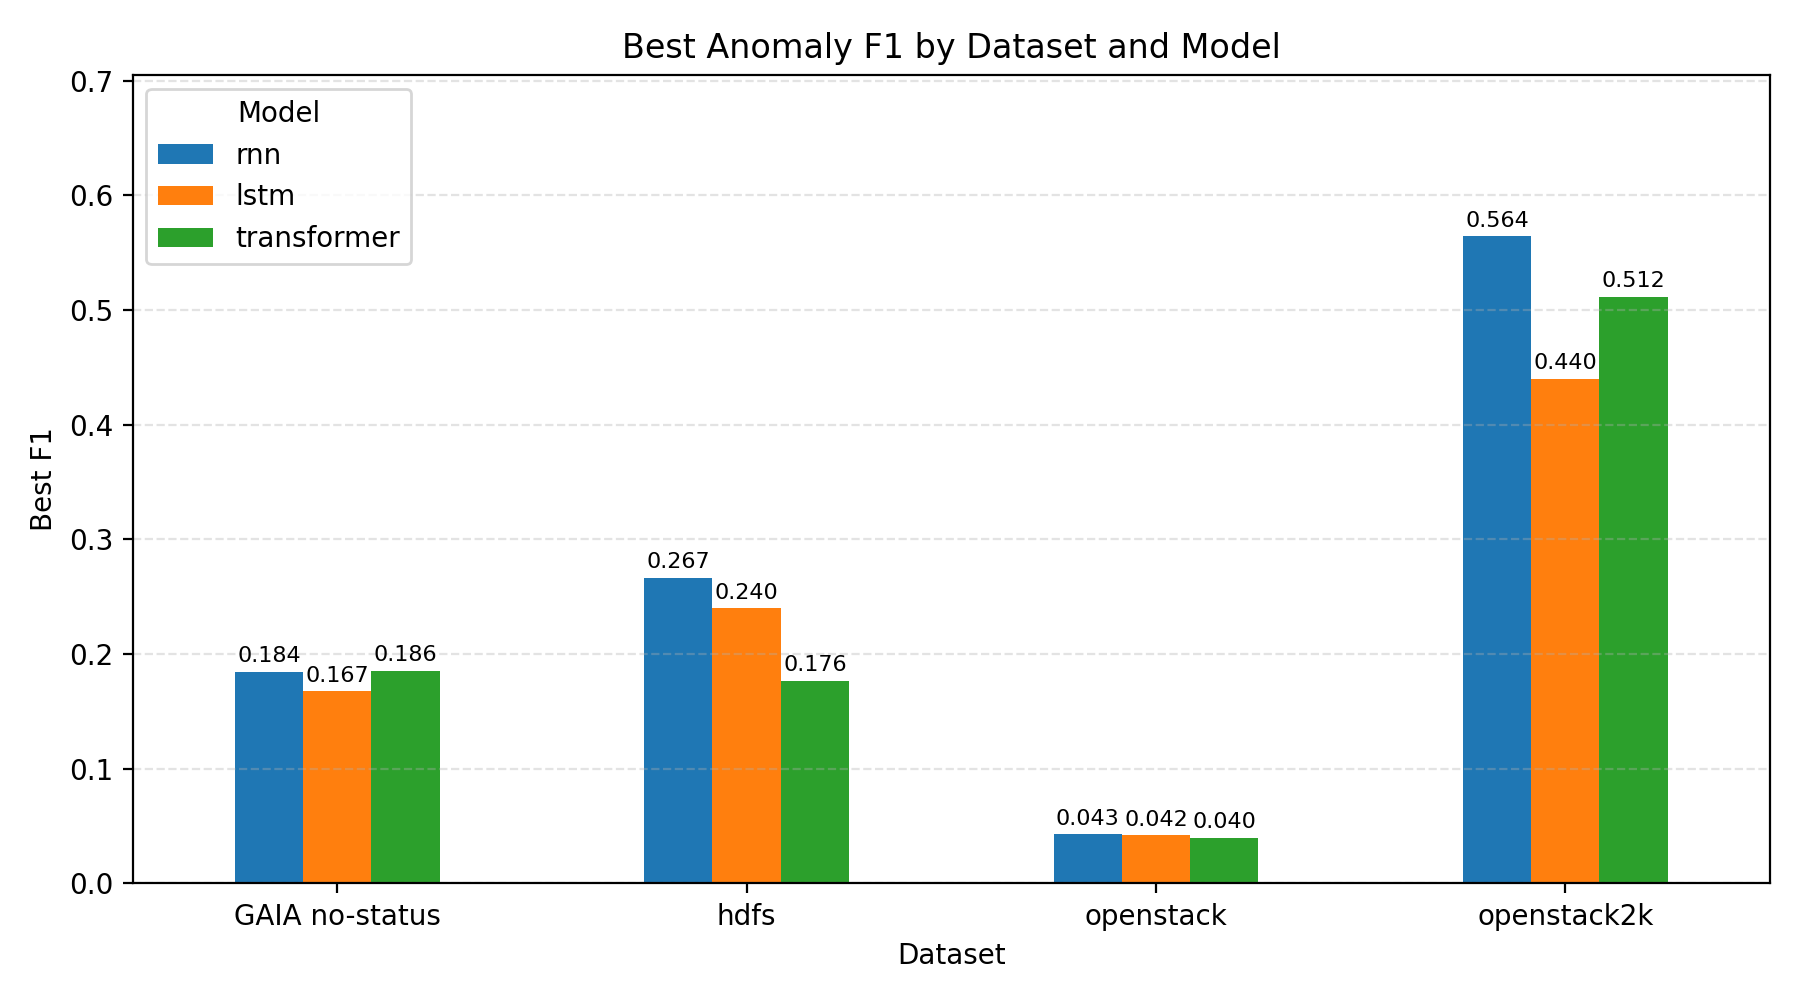
\includegraphics[width=0.70\textwidth]{outputs/final_report/figures/best_f1_by_dataset_model.png}
\caption{Best anomaly F1 by dataset and model. Higher is better.}
\label{fig:best-f1}
\end{figure}

\FloatBarrier
\subsection{Accuracy Can Be Misleading}

The OpenStack result is the clearest example. All models get about 98.6\% next-event accuracy, but the anomaly F1 is only around 0.04. This means the model learned common normal transitions, but it did not separate the rare anomalous VM-instance behavior well.

Figure \ref{fig:accuracy-f1} compares next-event accuracy and anomaly F1 for the best run of each dataset/model pair. Each point is one dataset and one model. Points on the right have high next-state prediction accuracy, while points near the top have better anomaly detection. The important part is that a point can be far right but still low, which means the model predicts common events well but still does not catch anomalies well.

\begin{figure}[!htbp]
\centering
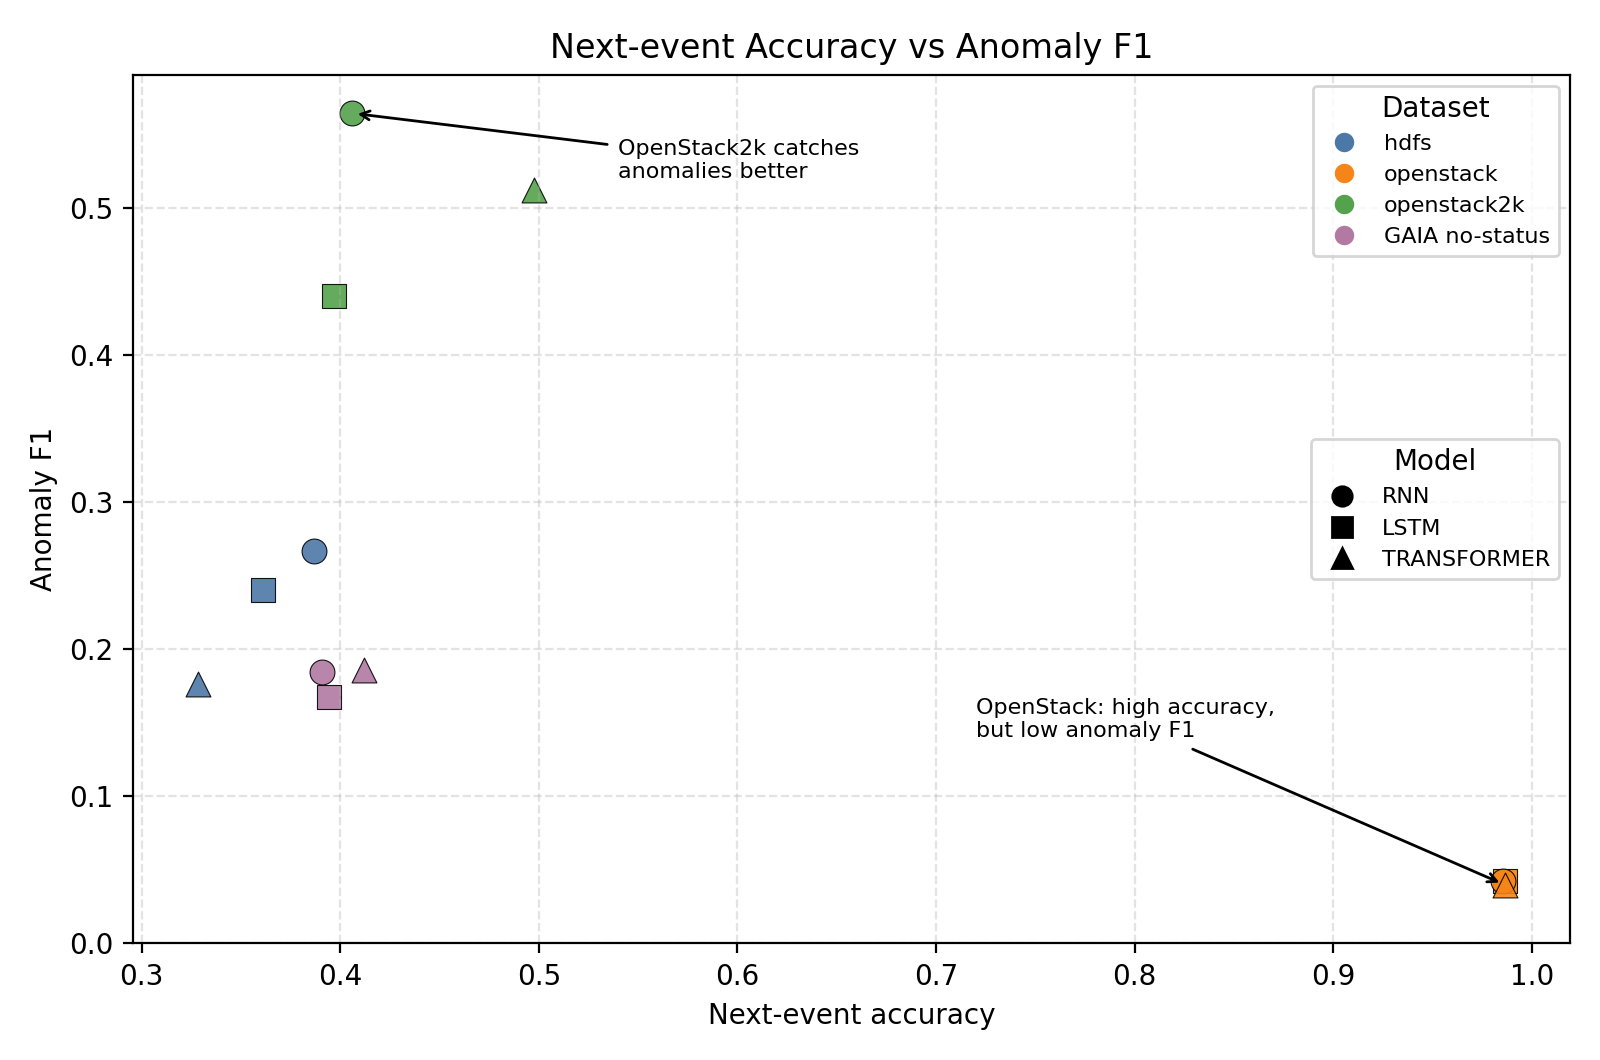
\includegraphics[width=0.78\textwidth]{outputs/final_report/figures/accuracy_vs_f1.png}
\caption{Next-event accuracy vs anomaly F1. Each point is the best run for one dataset/model pair.}
\label{fig:accuracy-f1}
\end{figure}

\FloatBarrier
\subsection{GAIA Status-Code Ablation}

GAIA was important because it looked more like product infrastructure traces. But it also showed a common experimental trap.

\begin{figure}[!htbp]
\centering
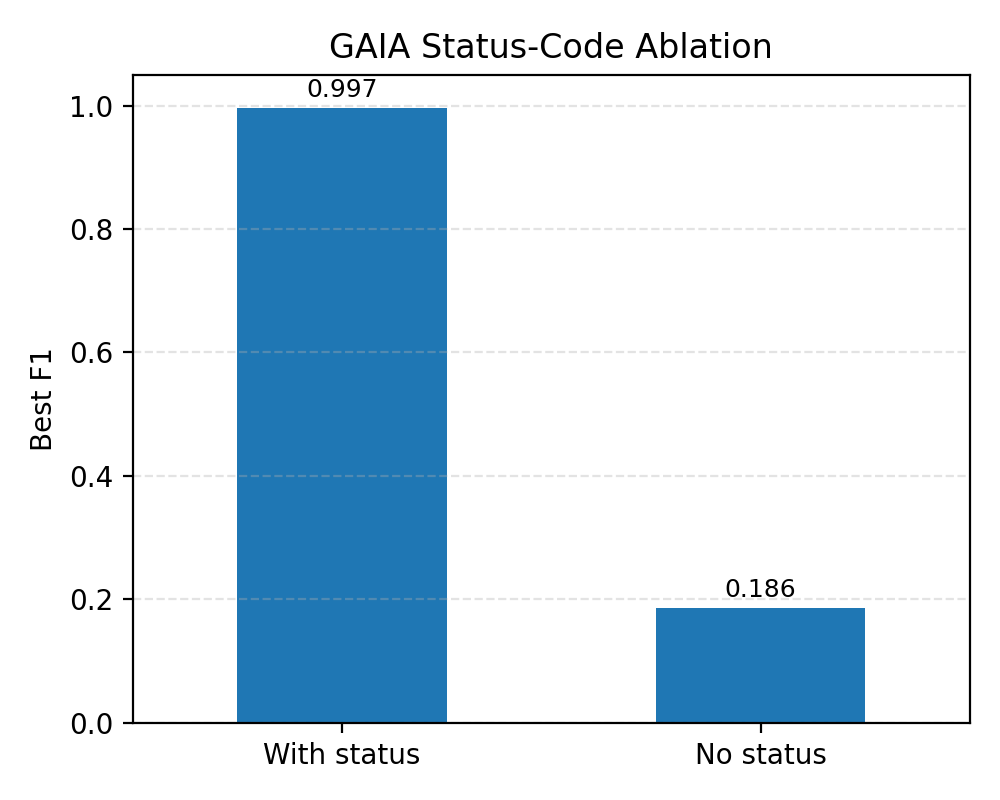
\includegraphics[width=0.48\textwidth]{outputs/final_report/figures/gaia_status_ablation.png}
\caption{GAIA ablation. Including status code leaks label information and makes the task too easy.}
\label{fig:gaia-ablation}
\end{figure}

At first, I included status code in the state token. Since the label was based on status code, the model almost got the answer directly. The best F1 was 0.997. After removing status code, the best F1 dropped to 0.186.

This does not mean GAIA is bad. It means feature design matters. The status-removed version is harder, but it is more honest because the model has to infer abnormal behavior from endpoint, service, duration, and message patterns.

\FloatBarrier
\subsection{Sequence Length}

I also tried different sequence lengths. On GAIA, sequence length 10 worked best in the no-status setting. Longer context did not automatically improve results.

\begin{figure}[!htbp]
\centering
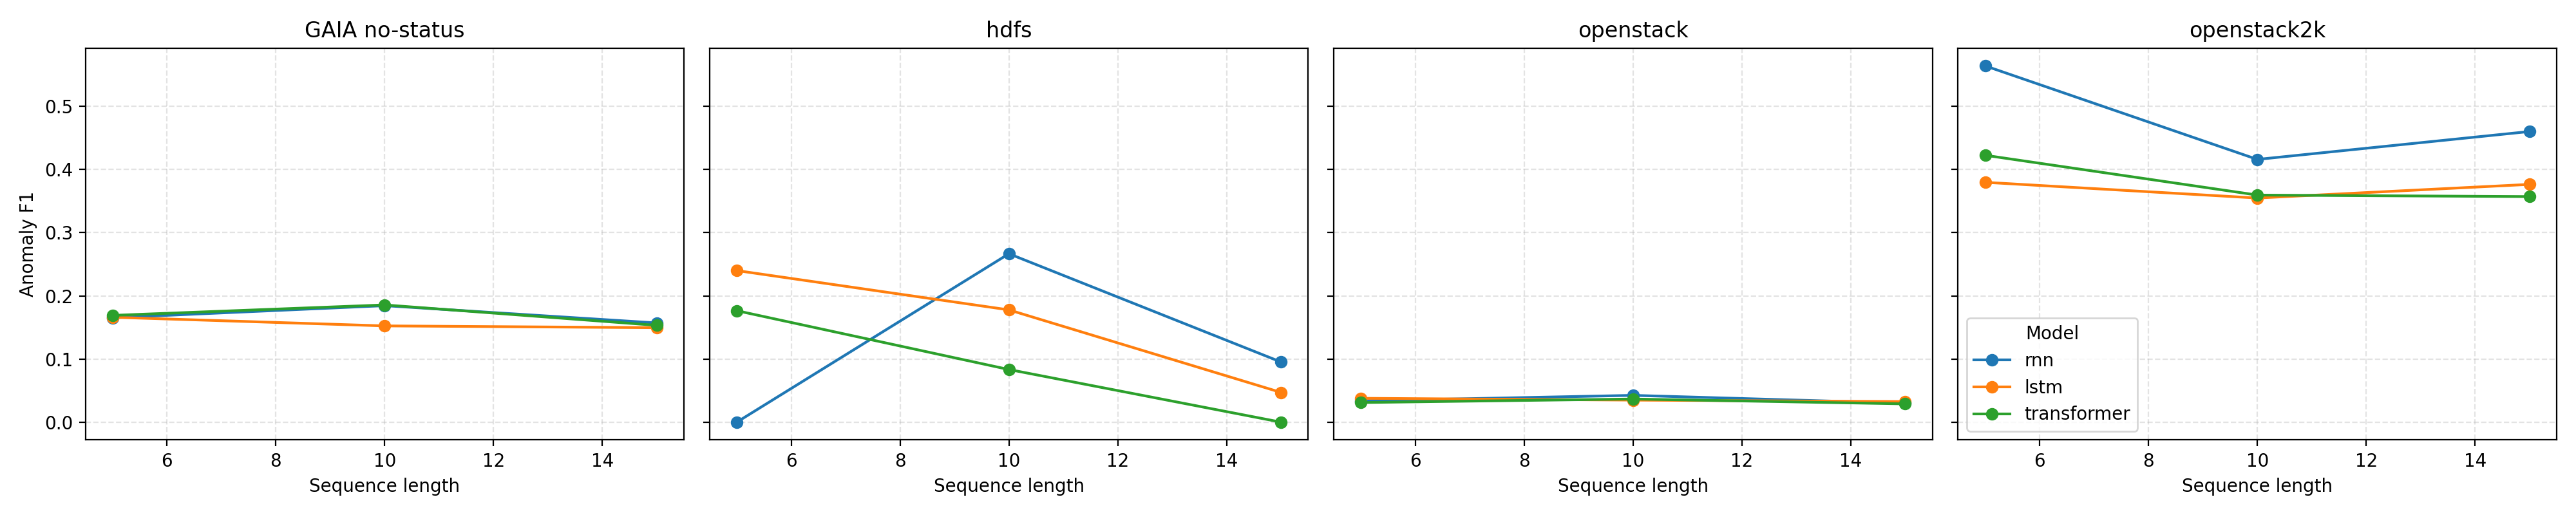
\includegraphics[width=0.82\textwidth]{outputs/final_report/figures/sequence_length_sweep.png}
\caption{Sequence length sweep. More context is not always better.}
\label{fig:sequence-sweep}
\end{figure}

\FloatBarrier
\section{Discussion}

The main thing I learned is that log anomaly detection is not only about choosing RNN vs LSTM vs Transformer. The dataset and state representation matter a lot.

OpenStack has very high prediction accuracy but very low F1 because the anomaly labels are sparse. OpenStack2k looks much better because the controlled anomalies directly affect the next-state prediction task. GAIA shows that product-infrastructure traces are useful, but also that we must be careful not to include the answer in the input.

The Transformer does not always win. In some settings, RNN is better. This makes sense because the datasets are small and the sequences are not always long enough for attention to show a big advantage. A simpler model can be enough when the state representation is already strong.

The most important limitation is that the current state representation is still simple. For example, GAIA duration is bucketed instead of using the exact latency. Future work could include richer numeric features, service-level aggregates, and better labels based on real incidents instead of only status code.

\section{Conclusion}

This project studied anomaly detection as a state-transition learning problem. Logs and traces were converted into state sequences. RNN, LSTM, and Transformer models were trained to predict the next state. High prediction loss was used as the anomaly score.

The results show that the idea can work, but only when the anomaly signal is represented in the sequence and aligned with the label. High next-event accuracy is not enough. OpenStack proves this clearly: accuracy is high, but F1 is very low. OpenStack2k shows that controlled anomalies are easier. GAIA shows both the promise of product-infrastructure traces and the danger of label leakage.

Overall, the project supports a practical conclusion: before trying more complex models, we should first make sure the state representation, labels, and evaluation setup are meaningful. Better features and better labels may improve anomaly detection more than simply switching from RNN to Transformer.

\begin{thebibliography}{10}

\bibitem{chandola2009survey}
V. Chandola, A. Banerjee, and V. Kumar,
``Anomaly detection: A survey,''
\emph{ACM Computing Surveys}, 2009.

\bibitem{xu2009consolelogs}
W. Xu, L. Huang, A. Fox, D. Patterson, and M. Jordan,
``Detecting large-scale system problems by mining console logs,''
in \emph{Proc. ACM SOSP}, 2009.

\bibitem{lou2010invariants}
J. Lou, Q. Fu, S. Yang, Y. Xu, and J. Li,
``Mining invariants from console logs for system problem detection,''
in \emph{Proc. USENIX ATC}, 2010.

\bibitem{du2017deeplog}
M. Du, F. Li, G. Zheng, and V. Srikumar,
``DeepLog: Anomaly detection and diagnosis from system logs through deep learning,''
in \emph{Proc. ACM CCS}, 2017.

\bibitem{meng2019loganomaly}
W. Meng, Y. Liu, Y. Zhu, S. Zhang, D. Pei, Y. Liu, Y. Chen, R. Zhang, S. Tao, P. Sun, and R. Zhou,
``LogAnomaly: Unsupervised detection of sequential and quantitative anomalies in unstructured logs,''
in \emph{Proc. IJCAI}, 2019.

\bibitem{guo2021logbert}
H. Guo, S. Yuan, and X. Wu,
``LogBERT: Log anomaly detection via BERT,''
in \emph{Proc. IJCNN}, 2021.

\bibitem{landauer2023dlsurvey}
M. Landauer, F. Skopik, M. Wurzenberger, W. Hotwagner, and A. Rauber,
``A critical review of common log data sets used for evaluation of sequence-based anomaly detection techniques,''
\emph{ACM Computing Surveys}, 2023.

\bibitem{loghub}
LogPAI,
``Loghub: A large collection of system log datasets,''
\url{https://github.com/logpai/loghub}.

\bibitem{gaia}
CloudWise,
``GAIA DataSet: Generic AIOps Atlas,''
\url{https://github.com/CloudWise-OpenSource/GAIA-DataSet}.

\end{thebibliography}

\end{document}
